\documentclass{standalone}
\usepackage{tikz}
\usetikzlibrary{shapes,arrows,positioning}
\begin{document}
  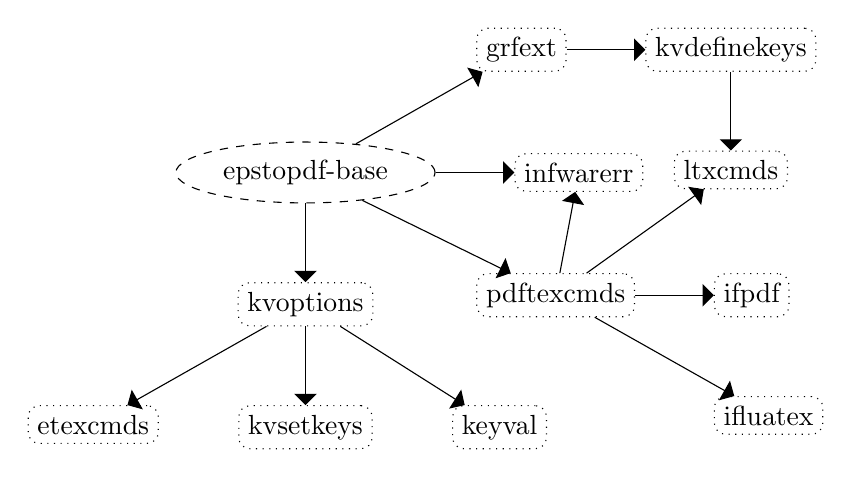
\begin{tikzpicture}
   \tikzset{main node/.style={rectangle, draw,
   		text centered, rounded corners}, }
   \tikzset{internal node/.style={rectangle, draw,dotted,
   		text centered, rounded corners}, }
   \tikzset{driver node/.style={ellipse, draw,dashed,
   		text centered}, }
   \tikzset{formato node/.style={rectangle, draw,dotted,
   		text centered}, }
   \tikzset{cfg node/.style={minimum size=1cm}, }
   \tikzset{linea/.style={-triangle 90},}
  
\node[driver node] (1) {epstopdf-base};
%\node (2) [right =of 1] {};
\node[internal node] (3) [ right =of 1] {infwarerr};
\node[internal node] (4) [above right =of 1] {grfext};
\node[internal node] (5) [below right =of 1] {pdftexcmds};
\node[internal node] (6) [below =of 1] {kvoptions};
\node[internal node] (7) [below right=of 6] {keyval};
\node[internal node] (8) [below =of 6] {kvsetkeys};
\node[internal node] (9) [below left=of 6] {etexcmds};
\node[internal node] (10) [right =of 4] {kvdefinekeys};
\node[internal node] (11) [below =of 10] {ltxcmds};
\node[internal node] (12) [right =of 5] {ifpdf};
\node[internal node] (13) [below right =of 5] {ifluatex};
\foreach \x /\y in{1/3,1/4,1/5,1/6,6/7,6/8,6/9,4/10,10/11,5/3,5/11,5/12,5/13}
\path[linea] (\x) edge node {} (\y);
% 
\end{tikzpicture}
\end{document}